\begin{appendix}

\chapter{Backpropagation Example}
\label{sec:bp_walkthrough}

This section describes an example of training a backpropagation network by using the algorithm shown in \ref{sec:backpropagation}. The network uses the sigmoid shown in section \ref{sec:activation} as activation function.

Similar examples can also be found in \cite{backpropagation_example} and \cite{backpropagation_example_2}.

\section{The Network Structure}

The network that is used in this example is shown in figure \ref{backpropagation_ex}. It contains an input layer with two neurons, one hidden layer with two neurons and an output layer with two neurons. The initial weight values are already initialised with random values between -1 and 1. It uses a learning rate of 0.25 and no bias element is used.

\begin{figure}[htbp]
	\vspace{0.5em}
	\begin{center}
		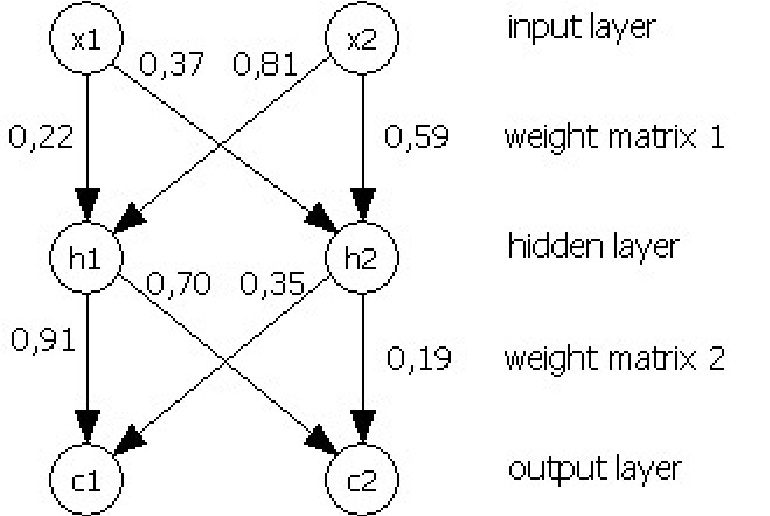
\includegraphics[width=0.55\columnwidth]{graphics/Backpropagation_ex}
	\end{center}
	\vspace{-1em}
	\caption{An example of a backpropagation network}
	\label{backpropagation_ex}
\end{figure}

\section{The Patterns to be Learnt}

The goal of this example is to learn the patterns shown in table \ref{pattern_learn}. The first output value $o_1$ indicates a flood attack with medium danger and the second value $o_2$ indicates a flood attack with high danger.

\begin{table}[htbp]
	\vspace{1.5em}
	\begin{center}
		\begin{tabular}{|l|l|l|l|}
		\hline
		\bf{$x_1$}&\bf{$x_2$}&\bf{$o_1$}&\bf{$o_2$}\\
		\hline
		1&1&0&1\\
		\hline
		1&0&1&0\\
		\hline
		0&1&1&0\\
		\hline
		0&0&0&0\\
		\hline
		\end{tabular}
	\end{center}
	\vspace{-1em}
	\caption{An example of a pattern set to be learnt}
	\label{pattern_learn}
\end{table}

\section{Step by Step Description}

\begin{enumerate}
    \item Calculate $c^L_p(i), p=1,...k_L$: \ \\

	Activate nodes in the hidden layer: \\

	Input of hidden neuron h1: $0,22*1 + 0,81*1 = 1,03$ \\
	Input of hidden neuron h2: $0,37*1 + 0,59*1 = 0,96$ \\
	Output of hidden neuron h1: $\frac{1}{1+\exp(-1,03)} = 0,736916$ \\
	Output of hidden neuron h2: $\frac{1}{1+\exp(-0,96)} = 0,723122$ \\

	Activate nodes in the output layer: \\

	Input of output neuron c1: $0,91*0,736916 + 0,35*0,7231218 = 0,923686$\\
	Input of output neuron c2: $0,70*0,736916 + 0,19*0,7231218 = 0,653234$\\
	Output of output neuron c1: $\frac{1}{1+\exp(-0,923686)} = {\bf 0,715793}$\\
	Output of output neuron c2: $\frac{1}{1+\exp(-0,653234)} = {\bf 0,657739}$\\


	\item Calculate $\delta^L_p, p=1,...,k_L$: \ \\

	Error value of output neuron c1: $(0,715793 - 0) * (0,715793) * (1 - 0,715793) = 0,145616$ \\
	Error value of output neuron c2: $(0,657739 - 1) * (0,657739) * (1 - 0,657739) = -0,077049$ \\

	\item For $q = L - 1$ to $1$ calculate $\delta^q_p, p=1,...,k_q$: \ \\

	Error value of hidden neuron h1: $ [(0,145616 * 0,91) + (-0,077049 * 0,70)] * (0,736916) * (1 - 0,736916) = 0,015233$ \\
	Error value of hidden neuron h2: $ [(0,145616 * 0,35) + (-0,077049 * 0,19)] * (0,723122) * (1 - 0,723122) = 0,007273$ \\

	\item Update weight vectors: \ \\

	Update weight matrix 1: \\

	w(x1, h1): $0,22 - 0,25 * (0,015233 * 1) = 0,216192$ \\
	w(x2, h1): $0,81 - 0,25 * (0,015233 * 1) = 0,806192$ \\
	w(x1, h2): $0,37 - 0,25 * (0,007273 * 1) = 0,368182$ \\
	w(x2, h2): $0,59 - 0,25 * (0,007273 * 1) = 0,588182$ \\

	Update weight matrix 2: \\

	w(h1, c1): $0,91 - 0,25 * (0,145616 * 0,736916) = 0,883173$ \\
	w(h2, c1): $0,35 - 0,25 * (0,145616 * 0,723122) = 0,323675$ \\
	w(h1, c2): $0,70 - 0,25 * (-0,077049 * 0,736916) = 0,714195$ \\
	w(h2, c2): $0,19 - 0,25 * (-0,077049 * 0,723122) = 0,203929$ \\

	\item Restart learning with next pattern.

\end{enumerate}

\chapter{Aircrack versus WepLab}
\label{sec:aircrack_weplab}

This section shows a comparison between Aircrack (v2.41) and WepLab (v0.1.15). The following tables present how many seconds are needed to break a 64 bit WEP key. All tests are performed on an Intel Centrino laptop with 1600 Mhz and 512 MB RAM running Ubuntu Linux with the kernel version 2.6.12.

The sign "-" indicates that the tool did not find a correct solution and the "s" stands for stopped. This is used in case the test took more than five minutes.

\section{Aircrack}

Aircrack was run by issuing: {\bf aircrack -f {\em fudge factor} -n 64 {\em file}}

Table \ref{aircrack} shows the test result of running aircrack. The numbers in the first line specify the fudge factor used.

\begin{table}[htbp]
	\begin{center}
		\begin{tabular}{|l|l|l|l|l|l|l|}
		\hline
		\bf{packets}&\bf{unique IVs} &\bf{2} &\bf{4} &\bf{8} &\bf{16} &\bf{32}\\
		\hline
		100.000&40.832&-&-&01:01&02:49&02:48\\
		\hline
		200.000&82.465&-&-&s&s&s\\
		\hline
		300.000&125.052&-&-&s&s&s\\
		\hline
		400.000&167.740&-&-&s&s&s\\
		\hline
		500.000&210.349&-&-&s&s&s\\
		\hline
		600.000&253.787&-&-&s&s&s\\
		\hline
		700.000&297.370&-&-&s&s&s\\
		\hline
		800.000&340.960&00:01&00:01&00:02&00:02&00:01\\
		\hline
		900.000&384.604&00:02&00:02&00:01&00:02&00:01\\
		\hline
		1.000.000&428.195&00:02&00:02&00:02&00:02&00:02\\
		\hline
		\end{tabular}
	\end{center}
	\vspace{-1em}
	\caption{Aircrack test results}
	\label{aircrack}
\end{table}

\section{WepLab}

WepLab was run by issuing: {\bf weplab -r -k 64 --perc {\em value} {\em file}}

Table \ref{weplab} shows the test result of running WepLab. The numbers in the first line specify the value used for the --perc parameter.

\begin{table}[htbp]
	\begin{center}
		\begin{tabular}{|l|l|l|l|l|l|l|}
		\hline
		\bf{packets}&\bf{unique IVs} &\bf{50} &\bf{70} &\bf{90}\\
		\hline
		100.000&40.832&s&s&s\\
		\hline
		200.000&82.465&-&s&s\\
		\hline
		300.000&125.052&-&s&s\\
		\hline
		400.000&167.740&-&04:20&s\\
		\hline
		500.000&210.349&-&-&s\\
		\hline
		600.000&253.787&-&s&s\\
		\hline
		700.000&297.370&-&-&s\\
		\hline
		800.000&340.960&00:05&00:08&00:57\\
		\hline
		900.000&384.604&00:02&00:02&00:03\\
		\hline
		1.000.000&428.195&-&00:03&00:03\\
		\hline
		\end{tabular}
	\end{center}
	\vspace{-1em}
	\caption{WepLab test results}
	\label{weplab}
\end{table}

\chapter{Tools}

Last visited on August 8th, 2006.

\begin{list}{}
	{
		\setlength{\labelwidth}{10em}
		\leftmargin\labelwidth \advance\leftmargin by \labelsep
		\renewcommand{\makelabel}[1]{\mbox{\textbf{#1}}\dotfill}
	}
	\item[Aircrack] \begin{list}{}
		{
			\setlength{\parsep}{0em}
			\setlength{\labelwidth}{4em}
			\leftmargin\labelwidth \advance\leftmargin by \labelsep
			\renewcommand{\makelabel}[1]{\mbox{#1}}
		}
		\item[Version:] 2.41
		\item[URL:] http://www.aircrack-ng.org/doku.php
		\item[OS:] Linux, Windows
	\end{list}
	\item[AirSnare] \begin{list}{}
		{
			\setlength{\parsep}{0em}
			\setlength{\labelwidth}{4em}
			\leftmargin\labelwidth \advance\leftmargin by \labelsep
			\renewcommand{\makelabel}[1]{\mbox{#1}}
		}
		\item[Version:] 1.5.0
		\item[URL:] http://home.comcast.net/~jay.deboer/airsnare/
		\item[OS:] Windows
	\end{list}
	\item[AirSnort] \begin{list}{}
		{
			\setlength{\parsep}{0em}
			\setlength{\labelwidth}{4em}
			\leftmargin\labelwidth \advance\leftmargin by \labelsep
			\renewcommand{\makelabel}[1]{\mbox{#1}}
		}
		\item[Version:] 0.2.7
		\item[URL:] http://airsnort.shmoo.com/
		\item[OS:] Linux, Windows
	\end{list}
	\item[Dwepcrack] \begin{list}{}
		{
			\setlength{\parsep}{0em}
			\setlength{\labelwidth}{4em}
			\leftmargin\labelwidth \advance\leftmargin by \labelsep
			\renewcommand{\makelabel}[1]{\mbox{#1}}
		}
		\item[Version:] 0.4
		\item[URL:] http://www.dachb0den.com/projects/dwepcrack.html
		\item[OS:] Linux
	\end{list}
	\item[Kismet] \begin{list}{}
		{
			\setlength{\parsep}{0em}
			\setlength{\labelwidth}{4em}
			\leftmargin\labelwidth \advance\leftmargin by \labelsep
			\renewcommand{\makelabel}[1]{\mbox{#1}}
		}
		\item[Version:] 2005.08.R1
		\item[URL:] http://www.kismetwireless.net/
		\item[OS:] Linux
	\end{list}
	\item[Netstumbler] \begin{list}{}
		{
			\setlength{\parsep}{0em}
			\setlength{\labelwidth}{4em}
			\leftmargin\labelwidth \advance\leftmargin by \labelsep
			\renewcommand{\makelabel}[1]{\mbox{#1}}
		}
		\item[Version:] 0.4.0
		\item[URL:] http://www.netstumbler.com/
		\item[OS:] Windows
	\end{list}
	\item[WepLab] \begin{list}{}
		{
			\setlength{\parsep}{0em}
			\setlength{\labelwidth}{4em}
			\leftmargin\labelwidth \advance\leftmargin by \labelsep
			\renewcommand{\makelabel}[1]{\mbox{#1}}
		}
		\item[Version:] 0.1.5
		\item[URL:] http://weplab.sourceforge.net/
		\item[OS:] Linux, Windows
	\end{list}
	\item[WIDZ] \begin{list}{}
		{
			\setlength{\parsep}{0em}
			\setlength{\labelwidth}{4em}
			\leftmargin\labelwidth \advance\leftmargin by \labelsep
			\renewcommand{\makelabel}[1]{\mbox{#1}}
		}
		\item[Version:] 1.5
		\item[URL:] http://www.loud-fat-bloke.co.uk/tools.html
		\item[OS:] Linux
	\end{list}
	\item[Wireless Snort] \begin{list}{}
		{
			\setlength{\parsep}{0em}
			\setlength{\labelwidth}{4em}
			\leftmargin\labelwidth \advance\leftmargin by \labelsep
			\renewcommand{\makelabel}[1]{\mbox{#1}}
		}
		\item[Version:] 2.4.3
		\item[URL:] http://snort-wireless.org/
		\item[OS:] Linux, Windows
	\end{list}
\end{list}

\chapter{Implementation}
\label{sec:implementation}

The implementation of this WIDS is a {\em proof of concept} and shows whether it is possible to use a neural network for intrusion detection. Since it combines the use of white lists and a neural network it is titled as a {\em hybrid approach}.

The program was created in Eclipse\footnote{Eclipse is available at: http://www.eclipse.org/} using a gnu c++ compiler\footnote{MinGW is available at: http://www.mingw.org/} version 3.4.2 for Windows.

It was tested on an Intel Centrino laptop with 1600 Mhz and 512 MB RAM running under Windows XP Professional SP2.

The final version of the code has 4266 lines and can be found on the delivered CD.


\end{appendix}
